\subsection{Objekt-Dateien einlesen}
Unter "`Datei->Öffnen"' kann eine Objekt-Datei geöffnet werden (siehe Abb.~\ref{fig:DateiOeffnen}).

\begin{figure}[H]
\centering
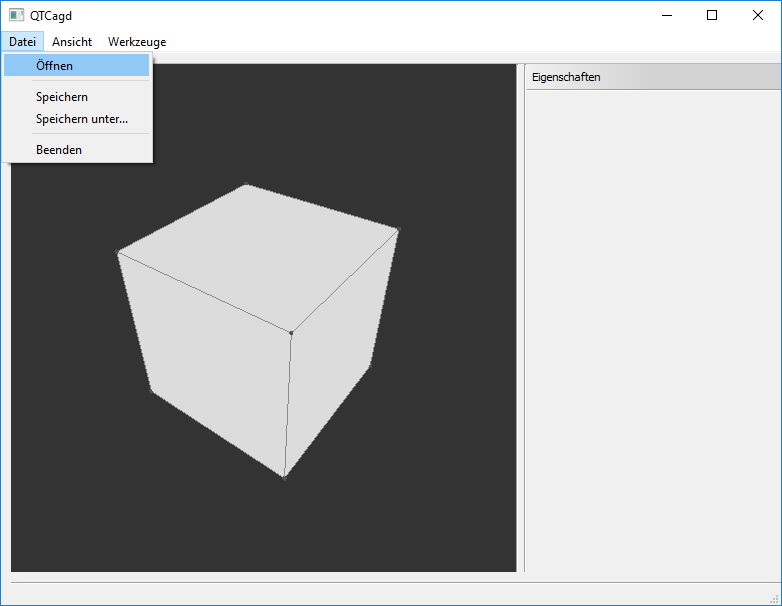
\includegraphics[scale=0.5]{content/pictures/0-DateiOeffnen}
\caption{}
\label{fig:DateiOeffnen}
\end{figure}

\subsection{Objekt-Dateien speichern}
Unter "`Datei->Speichern"' oder mit "`Datei->Speichern unter..."' kann eine Objekt-Datei gespeichert werden (siehe Abb.~\ref{fig:DateiSpeichern}).

\begin{figure}[H]
	\centering
	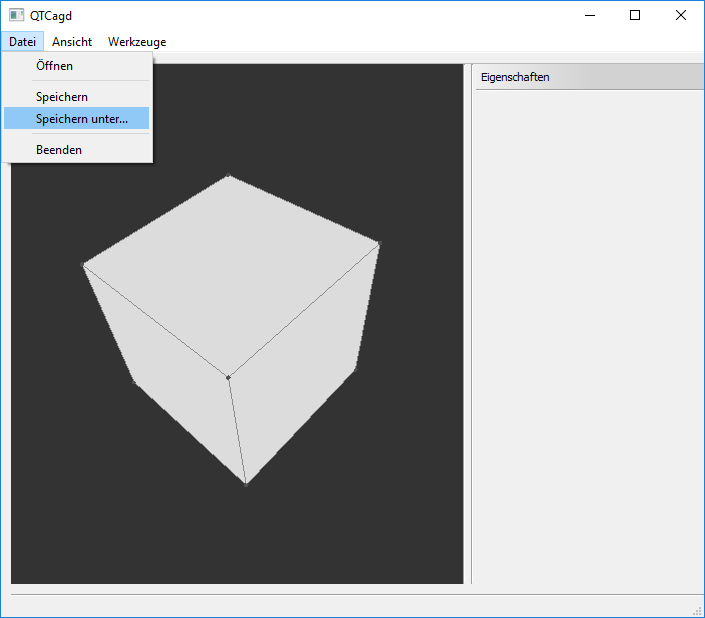
\includegraphics[scale=0.5]{content/pictures/1-DateiSpeichern}
	\caption{}
	\label{fig:DateiSpeichern}
\end{figure}

\subsection{Ansichtsmodi}
Es können 3 Ansichtsmodi aktiviert werden und zwar der "`Vertex Mode"', der "`Edge Mode"' oder der "`Face Mode"' (siehe Abb.~\ref{fig:Ansichtsmodi}).\\
Punkte können im "`Vertex Mode"' bearbeitet werden.\\
Kanten können im "`Edge Mode"' bearbeitet werden.\\
Flächen können im "`Face Mode"' bearbeitet werden.

\begin{figure}[H]
	\centering
	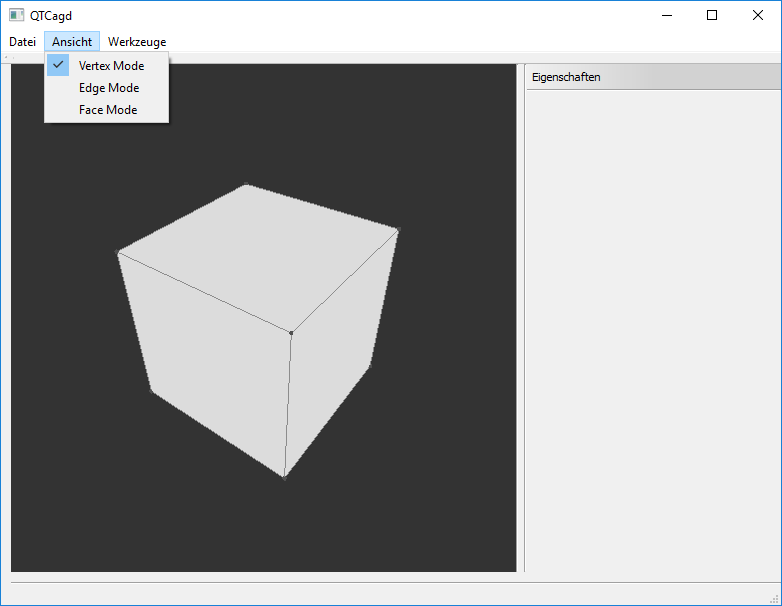
\includegraphics[scale=0.5]{content/pictures/2-Ansichtsmodi}
	\caption{}
	\label{fig:Ansichtsmodi}
\end{figure}

\subsection{Objekte selektieren}
Mit der Linken Maustaste können Grafikobjekte wie Punkte oder Kanten selektiert werden.\\
Mit Strg + Linke Maustaste kann eine Gruppe von Objekten selektiert werden.\\
Die Selektierten Objekte sind orange gefärbt (siehe Abb.~\ref{fig:ObjekteSelektieren}).\\
Mit der Rechten Maustaste kann das ganze Mesh gedreht werden.\\

\begin{figure}[H]
	\centering
	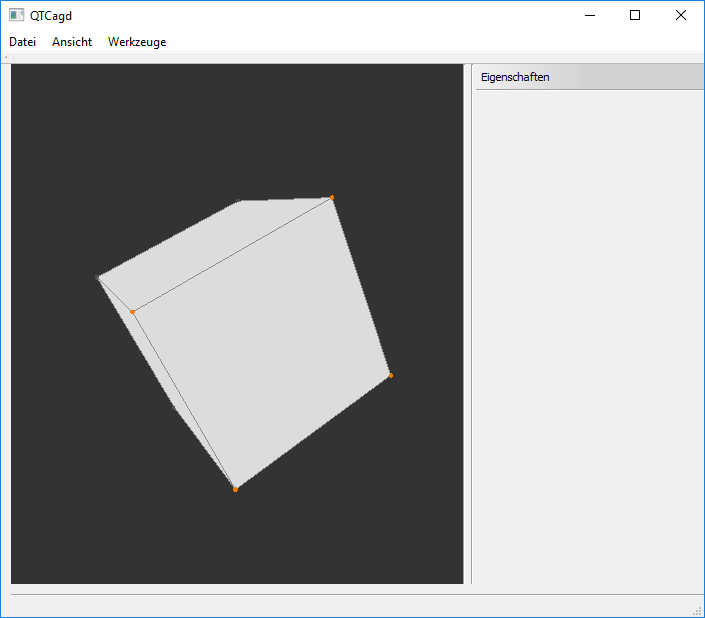
\includegraphics[scale=0.5]{content/pictures/3-ObjekteSelektieren}
	\caption{}
	\label{fig:ObjekteSelektieren}
\end{figure}

\subsection{Punkte verschieben}
Selektierte Punkte können mit gedrückter (linker) Maustaste und gleichzeitig gedrückter Alt-Taste verschoben werden.\\
Wird dabei die Taste einer Achse gedrückt (z.B. die X-Taste), so verschiebt sich die Selektion nur um die entsprechende Achse.\\
Ein selektierter Punkt kann auch mit den Spinboxen "`X-Koordinate"', "`Y-Koordinate"' und "`Z-Koordinate"' im "`Eigenschaften"' Menü verschoben werden (siehe Abb.~\ref{fig:PunkteVerschieben}).

\begin{figure}[H]
	\centering
	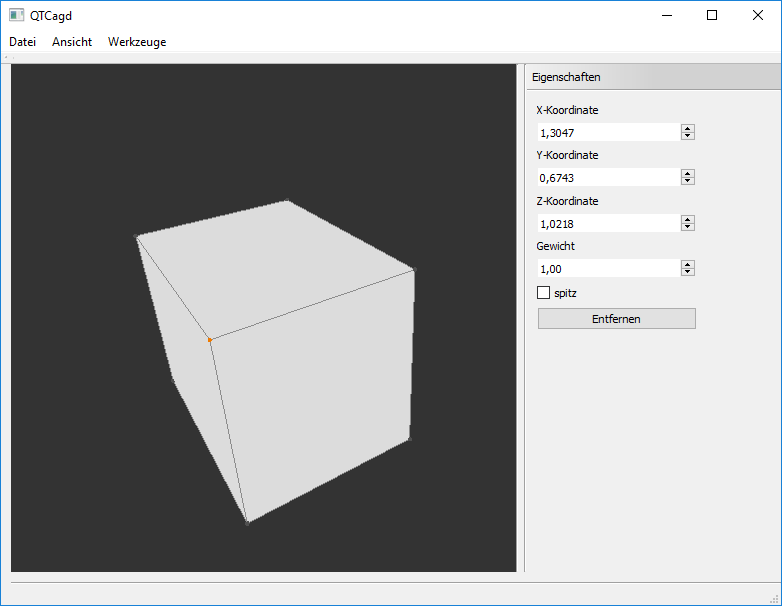
\includegraphics[scale=0.5]{content/pictures/4-PunkteVerschieben}
	\caption{}
	\label{fig:PunkteVerschieben}
\end{figure}

\subsection{Objekte löschen}
Selektierte Punkte, Kanten oder Flächen können mit der "`Entf"'-Taste gelöscht werden.\\
Ein selektiertes Objekt kann auch mit den Button "`Entfernen"' im "`Eigenschaften"' Menü gelöscht werden (siehe Abb.~\ref{fig:PunkteLoeschen}).

\begin{figure}[H]
	\centering
	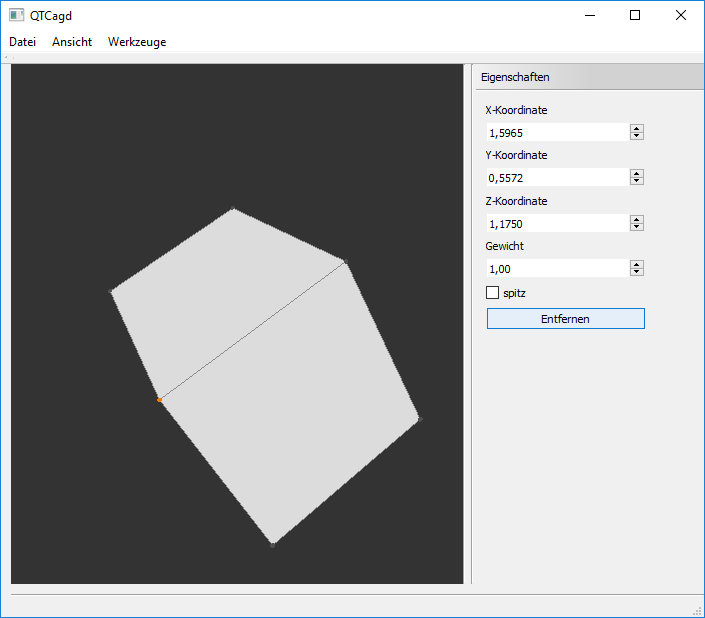
\includegraphics[scale=0.5]{content/pictures/5-PunkteLoeschen}
	\caption{}
	\label{fig:PunkteLoeschen}	
\end{figure}

\subsection{Punkte gewichten}
Ein selektierter Punkt kann mit der Spinbox "`Gewicht"' im "`Eigenschaften"' Menü gewichtet werden (siehe Abb.~\ref{fig:PunkteGewichten}).

\begin{figure}[H]
	\centering
	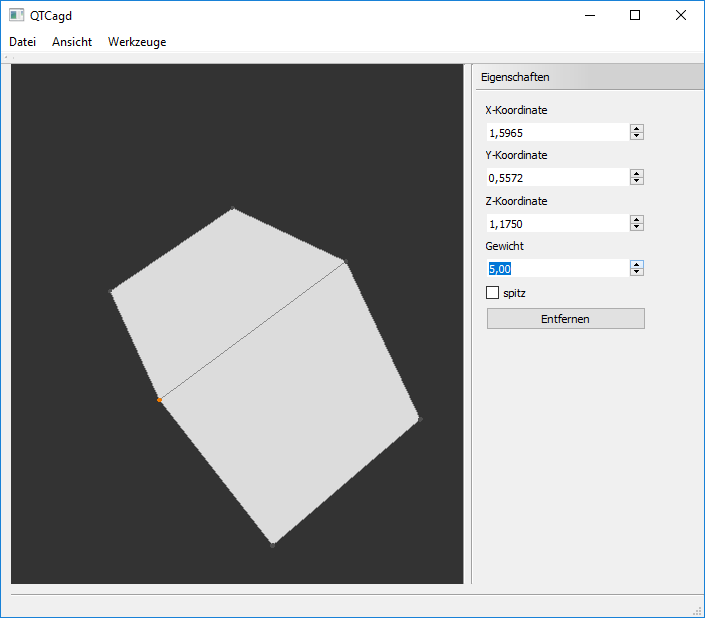
\includegraphics[scale=0.5]{content/pictures/6-PunkteGewichten}
	\caption{}
	\label{fig:PunkteGewichten}
\end{figure}

\subsection{Punkte und Kanten scharf setzen}
Ein selektierter Punkt oder eine selektierte Kante kann mit der Checkbox "`spitz"' bzw. "`scharf"' im "`Eigenschaften"' Menü scharf gesetzt werden (siehe Abb.~\ref{fig:Punkte-KantenScharfSetzen}).\\
Die Taste "`A"' setzt alle Kanten auf scharf.\\
Die Taste "`D"' setzt alle Kanten auf nicht scharf.\\

\begin{figure}[H]
	\centering
	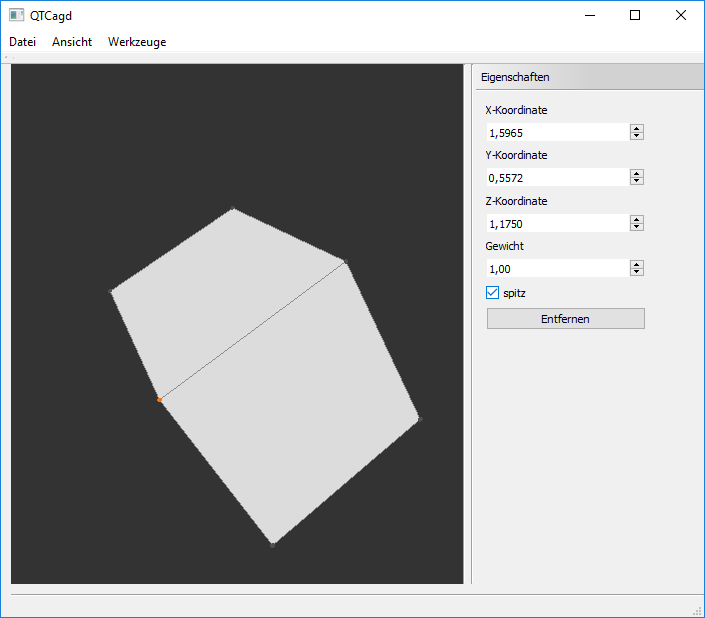
\includegraphics[scale=0.5]{content/pictures/7-Punkte-KantenScharfSetzen}
	\caption{}
	\label{fig:Punkte-KantenScharfSetzen}
\end{figure}

\subsection{Mesh mit Catmull-Clark unterteilen}
Unter "`Werkzeuge->Catmull-Clark"' wird das "`Catmull-Clark Subdivision"' Menü geöffnet.\\
Der Slider "`Level of Detail"' zeigt das Mesh in dem eingestellten Level of Detail an.\\
Der Button "`Anwenden"' unterteilt das Mesh (siehe Abb.~\ref{fig:MeshCatmullClark}).

\begin{figure}[H]
	\centering
	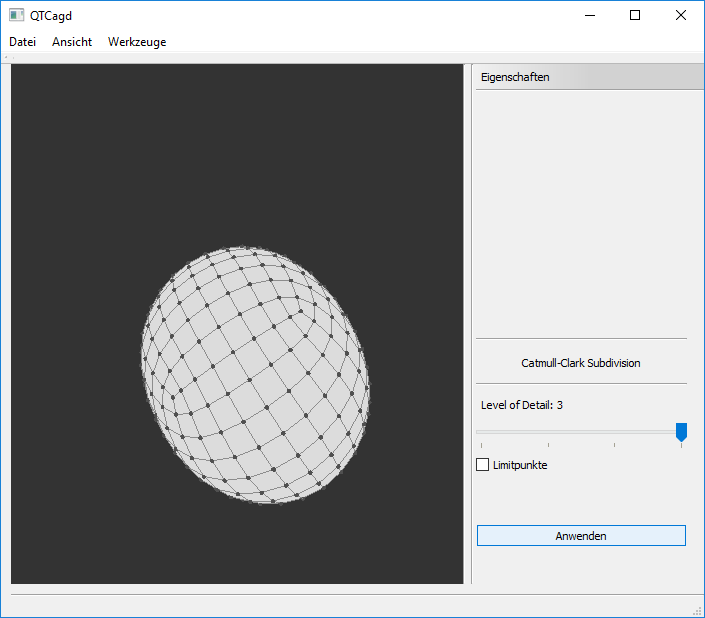
\includegraphics[scale=0.5]{content/pictures/8-MeshCatmullClark}
	\caption{}
	\label{fig:MeshCatmullClark}
\end{figure}

\subsection{Konsistenzprüfung und Statistik}
Mit der Taste "`T"' kann ein Mesh auf Fehler untersucht werden und die Statistik angezeigt werden (siehe Abb.~\ref{fig:TestStatistik}).\\
Au\ss{}erdem wird nach jeder Iteration Catmull-Clark automatisch auf Fehler untersucht.

\begin{figure}[H]
	\centering
	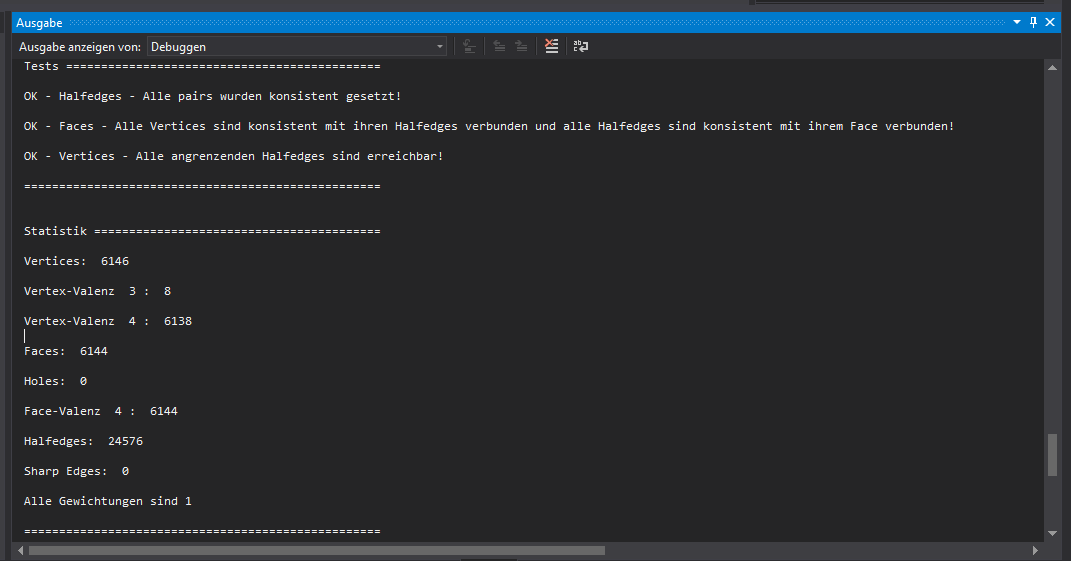
\includegraphics[scale=0.5]{content/pictures/9-TestStatistik}
	\caption{Konsistenzprüfung und Statistik für ein Dreieck}
	\label{fig:TestStatistik}
\end{figure}
